% ------------------------------------------------------------------------
% Artigo 
% ------------------------------------------------------------------------

% Carga de parâmetros



\documentclass[
	% -- opções da classe memoir --
	article,			        % indica que é um artigo acadêmico
	11pt,				          % tamanho da fonte
	oneside,			        % para impressão apenas no verso. Oposto a twoside
	a4paper,			        % tamanho do papel. 
	english,			        % idioma adicional para hifenização
	brazil,				        % o último idioma é o principal do documento
	sumario=tradicional
]{abntex2}\usepackage[]{graphicx}\usepackage[]{color}
%% maxwidth is the original width if it is less than linewidth
%% otherwise use linewidth (to make sure the graphics do not exceed the margin)
\makeatletter
\def\maxwidth{ %
  \ifdim\Gin@nat@width>\linewidth
    \linewidth
  \else
    \Gin@nat@width
  \fi
}
\makeatother

\definecolor{fgcolor}{rgb}{0.345, 0.345, 0.345}
\newcommand{\hlnum}[1]{\textcolor[rgb]{0.686,0.059,0.569}{#1}}%
\newcommand{\hlstr}[1]{\textcolor[rgb]{0.192,0.494,0.8}{#1}}%
\newcommand{\hlcom}[1]{\textcolor[rgb]{0.678,0.584,0.686}{\textit{#1}}}%
\newcommand{\hlopt}[1]{\textcolor[rgb]{0,0,0}{#1}}%
\newcommand{\hlstd}[1]{\textcolor[rgb]{0.345,0.345,0.345}{#1}}%
\newcommand{\hlkwa}[1]{\textcolor[rgb]{0.161,0.373,0.58}{\textbf{#1}}}%
\newcommand{\hlkwb}[1]{\textcolor[rgb]{0.69,0.353,0.396}{#1}}%
\newcommand{\hlkwc}[1]{\textcolor[rgb]{0.333,0.667,0.333}{#1}}%
\newcommand{\hlkwd}[1]{\textcolor[rgb]{0.737,0.353,0.396}{\textbf{#1}}}%

\usepackage{framed}
\makeatletter
\newenvironment{kframe}{%
 \def\at@end@of@kframe{}%
 \ifinner\ifhmode%
  \def\at@end@of@kframe{\end{minipage}}%
  \begin{minipage}{\columnwidth}%
 \fi\fi%
 \def\FrameCommand##1{\hskip\@totalleftmargin \hskip-\fboxsep
 \colorbox{shadecolor}{##1}\hskip-\fboxsep
     % There is no \\@totalrightmargin, so:
     \hskip-\linewidth \hskip-\@totalleftmargin \hskip\columnwidth}%
 \MakeFramed {\advance\hsize-\width
   \@totalleftmargin\z@ \linewidth\hsize
   \@setminipage}}%
 {\par\unskip\endMakeFramed%
 \at@end@of@kframe}
\makeatother

\definecolor{shadecolor}{rgb}{.97, .97, .97}
\definecolor{messagecolor}{rgb}{0, 0, 0}
\definecolor{warningcolor}{rgb}{1, 0, 1}
\definecolor{errorcolor}{rgb}{1, 0, 0}
\newenvironment{knitrout}{}{} % an empty environment to be redefined in TeX

\usepackage{alltt}


% ---
% PACOTES
% ---

% ---
% Pacotes fundamentais 
% ---
\usepackage{lmodern}			    % Usa a fonte Latin Modern
\usepackage[T1]{fontenc}		  % Selecao de codigos de fonte.
\usepackage[utf8]{inputenc}		% Codificacao do documento (conversão automática dos acentos)
\usepackage{indentfirst}   		% Indenta o primeiro parágrafo de cada seção.
\usepackage{nomencl}  		  	% Lista de simbolos
\usepackage{color}				    % Controle das cores
\usepackage{graphicx}			    % Inclusão de gráficos
\usepackage{microtype} 			  % para melhorias de justificação
\usepackage{amsmath}
\usepackage{amssymb}
\usepackage{amsfonts}
\usepackage{float}
\usepackage[brazilian,hyperpageref]{backref}	 % Paginas com as citações na bibl
\usepackage[alf]{abntex2cite}	% Citações padrão ABNT
\usepackage{everypage}
\usepackage{fourier}
\usepackage{multirow}
\usepackage{hyperref}
\AddEverypageHook{DRAFT VERSION}

% ---

% ---
% Configurações do pacote backref
% Usado sem a opção hyperpageref de backref
\renewcommand{\backrefpagesname}{Citado na(s) página(s):~}
% Texto padrão antes do número das páginas
\renewcommand{\backref}{}
% Define os textos da citação
\renewcommand*{\backrefalt}[4]{
	\ifcase #1 %
		Nenhuma citação no texto.%
	\or
		Citado na página #2.%
	\else
		Citado #1 vezes nas páginas #2.%
	\fi}%
% ---

% ---
% Informações de dados para CAPA e FOLHA DE ROSTO
% ---
\titulo{Jogos cooperativos na\\ gestão da cadeia de suprimentos}

\author{João B. G. Brito, \emph{Esp.}   \\   
    \href{mailto:jbgb@uol.com.br}{jbgb@uol.com.br} 
  \and {Michel J. Anzanello, \emph{Phd}} \\
    \href{mailto:michel.anzanello@gmail.com}{michel.anzanello@gmail.com}
}

\date{\today}

\instituicao{
    Universidade Federal do Rio Grande do Sul -- UFRGS\\
    Escola de Engenharia de Produção -- Programa de Pós-graduação
}

\local{Av. Osvaldo Aranha, 99 – 5º andar, CEP: 90035-190, Porto Alegre/RS}

% ---
% Configurações de aparência do PDF final

% alterando o aspecto da cor azul
\definecolor{blue}{RGB}{41,5,195}

% informações do PDF
\makeatletter
\hypersetup{
     	%pagebackref=true,
		pdftitle={\@title}, 
		pdfauthor={\@author},
    	pdfsubject={\@title},
	    pdfcreator={\@author},
  	pdfkeywords={Teoria dos jogos cooperativos}
                {Gestão da cadeia de suprimentos}
                {Shapley value},
   	 colorlinks=true,       	  % false: boxed links; true: colored links
     	linkcolor=blue,          	% color of internal links
    	citecolor=blue,        		% color of links to bibliography
    	filecolor=magenta,      	% color of file links
		urlcolor=blue,
		bookmarksdepth=4
}
\makeatother
% --- 

% compila o indice
% ---
\makeindex
% ---

% ---
% Altera as margens padrões
% ---
\setlrmarginsandblock{3cm}{3cm}{*}
\setulmarginsandblock{3cm}{3cm}{*}
\checkandfixthelayout
% ---

% --- 
% Espaçamentos entre linhas e parágrafos 
% --- 

% O tamanho do parágrafo é dado por:
\setlength{\parindent}{1.3cm}

% Controle do espaçamento entre um parágrafo e outro:
\setlength{\parskip}{0.2cm}  % tente também \onelineskip

% Espaçamento simples
\SingleSpacing

% ----
% Início do documento
% ----
\IfFileExists{upquote.sty}{\usepackage{upquote}}{}
\begin{document}

% Seleciona o idioma do documento (conforme pacotes do babel)
%\selectlanguage{english}
\selectlanguage{brazil}

% Retira espaço extra obsoleto entre as frases.
\frenchspacing 

% ----------------------------------------------------------
% ELEMENTOS PRÉ-TEXTUAIS
% ----------------------------------------------------------

%---
%
% Se desejar escrever o artigo em duas colunas, descomente a linha abaixo
% e a linha com o texto ``FIM DE ARTIGO EM DUAS COLUNAS''.
%
%---
% página de titulo
\maketitle


% resumo em português
\begin{resumoumacoluna}
% Contextualização: 
% Gap:
% Proposta: 
% Metodologia
% Resultados
% Conclusão 
No ambiente da cadeia de suprimentos (CS) as decisões de cada organização tendem a refletir nos seus elos. A análise dessas interações é importante para avaliar a colaboração entre seus membros, sugerir acordos e buscar o equilíbrio mais rentável. O presente artigo busca a equalização da contribuição marginal em consonância com axiomas de justiça oferecidos pelo emprego da teoria dos jogos cooperativos (TJC). A proposta é oferecer uma solução computacional gratuita e \emph{on-line} como interface de simulações do algoritmo \emph{Shapley Value}. A aplicação dispõe de um mapa para apontar a geolocalização de cada membro; painel com ocorrências para informar a contribuição marginal de cada relação, e área de apresentação dos resultados. O \emph{Shapley Value} retorna a razão justa de participação de cada componente na conjectura de todas as conexões --- cooperações --- possíveis. A proposta inicia com a apreciação dos conceitos da TJC na ambiência da Gestão da Cadeia de Suprimentos (GCS); o artigo afunila no estudo do método, e por fim, a lacuna é atendida pela implementação. A solução advém \texttt{(adicionar os resultados)}. Conclui--se que a adoção do \emph{Shapley Value} tem potencial de instrumentar apoio na definição de diretrizes da GCS, pois seu emprego oferece recursos para racionalizar relacionamentos, estratégias conflitantes e colaborativas.

 \vspace{\onelineskip}
 
 \noindent
 \textbf{Palavras-chave}: Agentes da cadeia de suprimentos. Otimização. Teoria dos Jogos. Shapley value.
\end{resumoumacoluna}

% ---

% ----------------------------------------------------------
% ELEMENTOS TEXTUAIS
% ----------------------------------------------------------
\textual

% \twocolumn[    		    
% ]      		% FIM DE ARTIGO EM DUAS COLUNAS
% ----------------------------------------------------------
% Introdução
% ----------------------------------------------------------
\section*{Introdução}
\addcontentsline{toc}{section}{Introdução}

Na profusão do mundo profissional organizações deparam-se com decisões difíceis de serem tomadas, tanto pela importância de suas consequências, quanto pelos resultados, muitas vezes, incertos \cite{Bekman.2009}. \citeonline{Nate.2012} destaca que a incerteza\footnote{Incerteza é o risco difícil de aferir \cite{Nate.2012}.} é usualmente interpretada como risco\footnote{Risco, conforme \citeonline{Knigth.1921}, é algo em que você pode colocar um preço.} --- uma imprecisão mensurável ---; \citeonline{Tversky.1972} é remissivo ao uso da intuição em cenários de incerteza, um artifício comum no processo de eliminação\footnote{Escolhas são analisadas como um probabilístico processo de sucessivas eliminações \cite{Tversky.1972}.} de opções, e para \citeonline{Mlodinow.2009}, tomar decisões e realizar avaliações sábias sobre condições de incerteza é uma habilidade rara. Porém, como qualquer habilidade, pode ser aperfeiçoada.

Na busca do julgamento perfeito, \citeonline{Condorcet.1785} formaliza o primeiro método de decisão ótima, utilizando probabilidade para quantificar opções. \citeonline{Davenport.2007} enfatizam o uso de ferramentas analíticas e de tomada de decisão para reduzir incertezas, agregar racionalidade e obter inteligência competitiva. Mas, para \citeonline{Kahneman.2012}, apesar de as pessoas em geral serem racionais, com decisões lógicas e sensatas, emoções como medo, apego e ódio explicam na maioria dos casos a irracionalidade das escolhas. Para \citeonline{Ariely.2009}, essa conduta define o conceito de economia comportamental, que considera como as pessoas se comportam e não como deveriam se comportar. 

É natural do ser humano estabelecer comparações para fundamentar suas decisões, sendo influenciado por forças racionais. Entretanto, as pessoas nem sempre são tão racionais, existindo diversas situações em que podemos contar com sua previsível irracionalidade \cite{Ariely.2012}. À vista disso, \citeonline{Mesquita.2009} defende o uso de ferramentas matemáticas que equacionem a predição de eventos de interação. Assim, introduz o uso da teoria dos jogos como mecanismo para entender comportamentos \cite[min.~2:17--2:37]{MesquitaTED.2009}.

Originalmente estabelecida em \citeyear{Cournot.1838} por \citeauthoronline{Cournot.1838} a teoria ganhou proeminência a partir do livro \emph{The Theory of Games and Economic Behavior} de \citeonline{Neumann.1947} que formalizou modelos matemáticos para estudo do comportamento econômico, nas interações entre agentes, em cenários de conflito ou cooperação. Transcendendo o ramo econômico, a teoria dos jogos ganhou aplicações em diversas áreas como: militar \cite{Haywood.1954,RAND.2004}, jurídica \cite{Rosa.2014}, biológica \cite{Smith.1982}, filosófica \cite{Lewis.2002} e política \cite{Levy.2003}. No ambiente empresarial \citeonline{Golden.1993} discutem a aplicação da teoria dos jogos em alianças de cooperação e competições estratégicas e \citeonline{Wang.2007} destaca sua adoção como uma ferramenta de apoio para selecionar estratégias. \citeonline{Lygero.1996} utilizam modelos da teoria para desenvolver controles híbridos em sistemas complexos, \citeonline{Shen.2002} emprega a teoria para decisões de programação em ambiente de produção e \citeonline{Huang.2001} utiliza abordagem na paridade das relações de publicidade da cadeia de suprimentos fabricante--varejista.

Para \citeonline{Campos.2012} não é raro que a aplicação dos conceitos de cadeia de suprimentos e logística\footnote{Logística é arte e ciência de mover as coisas de um lugar para outro e armazená-las ao longo do caminho \cite[p.~370]{Fawcett.2000}.} ocorra em um contexto multidisciplinar incorporando conhecimentos das áreas de custo, informática, estatística e matemática. \citeonline{Ayers.2006} delineia uma cadeia de suprimentos como um conjunto de empresas e pessoas que se relacionam trocando informações e produtos. Já o processo de GCS compreende atividades de decisão relacionadas à organização deste ambiente \cite{Fredendall.2001} e abrange planejamento, controle e coordenação dos canais de distribuição (fornecedores, prestadores de serviço, intermediários, clientes) \cite{Panitz.2007}. No âmbito dessa conjuntura, a chave da cooperação entre empresas está em conseguir a unidade de motivação pelo alinhamento de incentivos \cite{Cao.2012}. 

Uma cadeia de suprimentos é beneficiada pela colaboração entre seus membros, que pode ocorrer pelo compartilhamento de informações, conhecimentos, custos, riscos e recompensas. Mesmo que as organizações constituam unidades autônomas, temos uma sequência ou rede de relações interdependentes que pode promover alianças estratégicas \cite{Chen.2004}. Em geral, a cooperação vem ganhando cada vez mais importância, principalmente em redes de alta complexidade \cite{Drechsel.2010} onde as decisões de cada um dos membros (agentes) afetam nas decisões dos demais e o acordo entre os agentes é a base da cooperação \cite{Young.1994}.

Estudos sobre a aplicação da teoria dos jogos cooperativos no GCS versam como principal questão o gerenciamento harmonioso das decisões entre os elos da cadeia \cite{Dobos.2010a}. O pressuposto está na existência de uma estrutura comum entre agentes na qual o ganho ou custo seja compartilhado, seguindo critérios de justiça definidos por axiomas \cite{Bezerra.2009}. \citeonline{Brink.2002} caracteriza a propriedade de justiça e eficiência pelo modelo de jogo cooperativo \emph{Shapley Value}. 

Introduzido em  \citeyear{Shapley.1952} por \citeauthoronline{Shapley.1952}, os mais recentes estudos do método --- análogo ou no domínio do GCS ---, abarcam soluções nas ambiências do desenvolvimento sustentável \cite{Bakr.2015}, Internet das Coisas \cite{Militano.2016,Kim.2016}, redes sociais \cite{Kim.2016}, distribuição de lucros\footnote{Pesquisa sobre distribuição de lucros no \href{https://prod.campusexpress.upenn.edu/}{Campus Express Alliance}.} 
\cite{Zhuang.2016}, gerenciamento de projetos \cite{Ding.2016}, análise de impacto econômico\footnote{Impacto da expansão do \href{http://www.pancanal.com/eng/maritime/routes.html}{Canal do Panamá} no mercado de contêineres.} \cite{Liu.2016}, grafos\footnote{Relação entre elementos de um conjunto \cite{Deza.2014} --- interação dos agentes em uma coalizão.} \cite{Khmelnitskaya.2016}, estudos na alocação de custos para \emph{e--commerce} \cite{Dong.2016}, logística \cite{DeVos.2016}, cooperação vertical e horizontal\footnote{\citeauthoronline{Defryn.2016} relatam um estudo de caso de cooperação logística horizontal no setor das frutas e produtos hortícolas frescos.} no gerenciamento de inventário e transporte \cite{DeVos.2016,Defryn.2016}.

O presente artigo é uma abordagem sobre a execução do modelo \emph{Shapley Value} para equacionar a contribuição marginal entre agentes de uma CS. Para tal fim, é proposta uma solução computacional gratuita e \emph{on-line}. Os exemplos são ilustrados por uma hipotética cadeia composta por três fornecedores que compartilham seus pontos de distribuição, um centro de apoio e o atendimento a um cliente.  O objetivo é balancear os custos itinerários, considerando todas as conexões possíveis no atendimento do cliente. A noção de justiça é alcançada pela aplicação \emph{Shapley Value} e viabilizada pela codificação do algoritmo na linguagem R\footnote{\citetext{R.2016}}. Ademais, a conclusão projeta novas lacunas com enlace para estudos em trabalhos futuros.

% ----------------------------------------------------------
% Estudo de caso
% ----------------------------------------------------------
\section{Estudo de caso}

Considerando uma coalizão, formada por três fornecedores, adiciona-se indivíduos, um de cada vez, dando a cada um uma contribuição marginal $v(S \cup \{i\})$ --- $v(S)$ para $S$ indivíduos. Na medida em que os custos são ponderados atinge-se uma noção de justiça.

\begin{knitrout}
\definecolor{shadecolor}{rgb}{0.969, 0.969, 0.969}\color{fgcolor}\begin{figure}[H]

{\centering 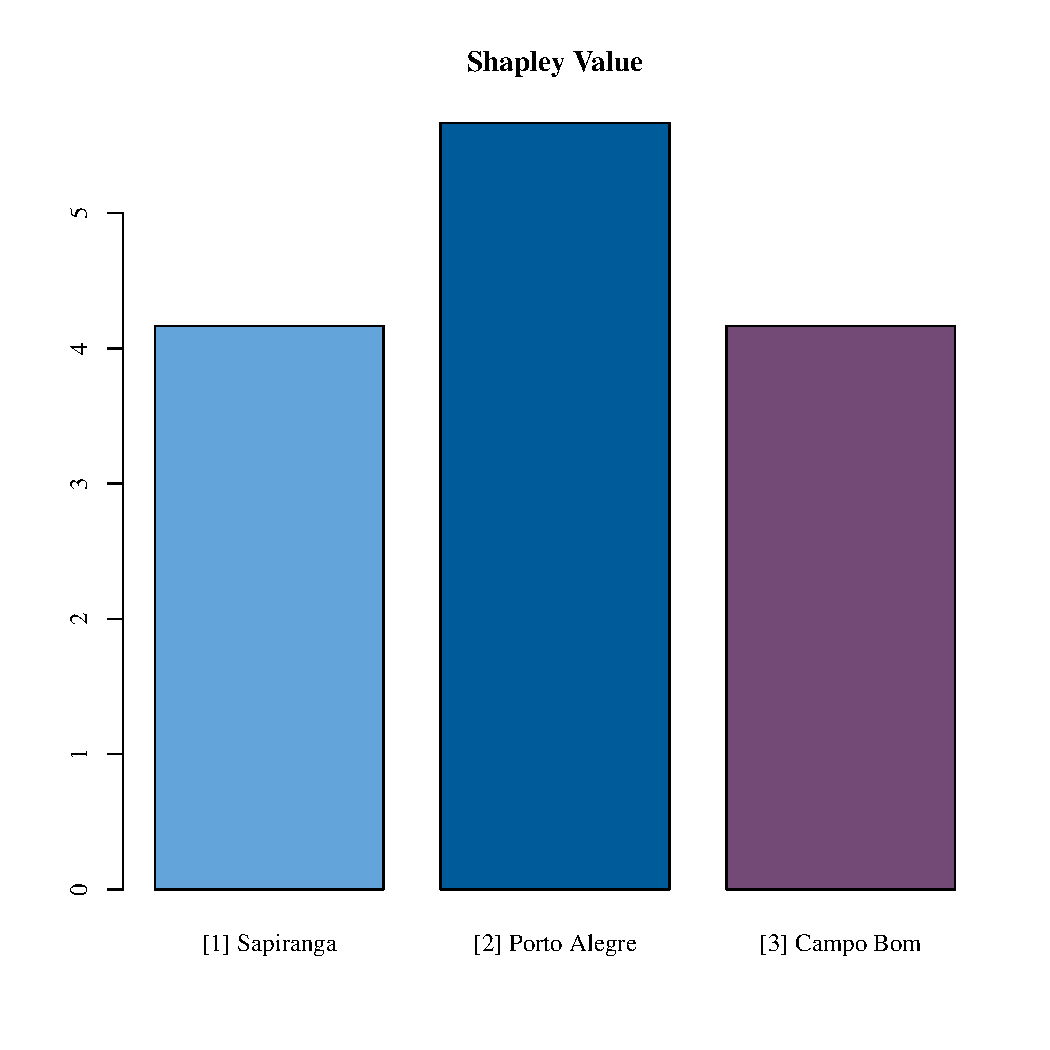
\includegraphics[width=\maxwidth]{figure/unnamed-chunk-2-1} 

}

\caption[Custo dos itinerários]{Custo dos itinerários}\label{fig:unnamed-chunk-2}
\end{figure}


\end{knitrout}

\begin{table}[!h]
  \centering
  \caption{Tabela de combinações de agentes e custo}
  \label{Tab1}
  \begin{tabular}{@{}cccccccccc@{}}
  \toprule
    $S$    & $\emptyset$ & $\{1\}$ & $\{2\}$ & $\{3\}$ & $\{1,2\}$ & $\{1,3\}$ & $\{2,3\}$ &     $\{1,2,3\}$ & $N$  \\ \midrule
    $v(S)$ & $0$         & $5$     & $8$     & $5$     & $10$      & $10$      & $10$      &     $14$        & $14$ \\ \bottomrule
  \end{tabular}
\end{table}

% ----------------------------------------------------------
% Shapley value
% ----------------------------------------------------------
\section{Shapley value}

\subsection{Conceito}

Sendo $\forall$ $S \neq \emptyset$ e $S \subset N$

\begin{equation}
  \label{eq:shaVal}
  \varphi _{i} = \sum_{S \subset N} \frac{(|s| - 1)!(n - |s|)!}{n!}[v(S)-v(S - i)]
\end{equation}

Shapley axiomas para $\varphi(v)$
\begin{enumerate}
  \item \textbf{Eficiência:} Toda alocação é distribuída sem disperídio $\sum_{i \in N} \varphi_i(v) - v(N)$.
  \item \textbf{Simetria:} Se $i$ e $j$ são tal que $v(S \cup \{i\}) = v(S \cup \{j\})$ para cada coalisão $S$ não contenha $i$ e $j$, então $\varphi_i (v) = \varphi_j (v)$
  \item \textbf{Linearidade:} Se dois agentes em uma coalizão, descritos pelas funões de ganho $\phi_i(v)$ e $\phi_i(w)$, são combinados, então os ganhos são correspondentes $\phi_i(v + w) = \phi_i(v) + \phi_i(w)$.
  \item \textbf{Zero jogador:} Quando um jogador não contribui na cooperação sua alocação é nula.
\end{enumerate}

\subsection{Aplicação no estudo de caso}

Para $i = 1$.

\begin{subequations}
  \tiny
  \begin{equation}
   \label{eq:shaValX1a}
    x_{[1]} = \frac{0!2!}{3!}(c(\{1\}) - c(\emptyset)) +
              \frac{1!1!}{3!}(c(\{1,2\}) - c(\{2\}) +
              \frac{1!1!}{3!}(c(\{1,3\}) - c(\{3\}) +
              \frac{2!0!}{3!}(c(\{1,2,3\}) - c(\{2,3\}) 
  \end{equation}

  $\therefore$

  \begin{equation}
   \label{eq:shaValX1b}
    x_{[1]} = \frac{2}{6}(c(\{5 - 0\}) +
              \frac{1}{6}(c(\{10 - 8\}) +
              \frac{1}{6}(c(\{10 - 5\}) +
              \frac{2}{6}(c(\{14 - 10\})
  \end{equation}

  $\therefore$

  \begin{equation}
   \label{eq:shaValX1c}
    x_{[1]} = \frac{25}{6} \cong 4,1667
   \end{equation}
\end{subequations}                  

Para $i = 2$.

\begin{subequations}
  \tiny
  \begin{equation}
   \label{eq:shaValX2a}
    x_{[2]} = \frac{0!2!}{3!}(c(\{2\}) - c(\emptyset)) +
              \frac{1!1!}{3!}(c(\{1,2\}) - c(\{1\}) +
              \frac{1!1!}{3!}(c(\{2,3\}) - c(\{3\}) +
              \frac{2!0!}{3!}(c(\{1,2,3\}) - c(\{1,3\}) 
  \end{equation}

  $\therefore$

  \begin{equation}
   \label{eq:shaValX2b}
    x_{[2]} = \frac{2}{6}(c(\{8 - 0\}) +
              \frac{1}{6}(c(\{10 - 5\}) +
              \frac{1}{6}(c(\{10 - 5\}) +
              \frac{2}{6}(c(\{14 - 10\})
  \end{equation}

  $\therefore$

  \begin{equation}
   \label{eq:shaValX2c}
    x_{[2]} = \frac{34}{6} \cong 5,6667
   \end{equation}
\end{subequations}                  

Para $i = 3$.

\begin{subequations}
  \tiny
  \begin{equation}
   \label{eq:shaValX3a}
    x_{[3]} = \frac{0!2!}{3!}(c(\{3\}) - c(\emptyset)) +
              \frac{1!1!}{3!}(c(\{1,3\}) - c(\{1\}) +
              \frac{1!1!}{3!}(c(\{2,3\}) - c(\{2\}) +
              \frac{2!0!}{3!}(c(\{1,2,3\}) - c(\{1,2\}) 
  \end{equation}
  
  $\therefore$
  
  \begin{equation}
   \label{eq:shaValX3b}
    x_{[3]} = \frac{2}{6}(c(\{5 - 0\}) +
              \frac{1}{6}(c(\{10 - 5\}) +
              \frac{1}{6}(c(\{10 - 8\}) +
              \frac{2}{6}(c(\{14 - 10\})
  \end{equation}

  $\therefore$

  \begin{equation}
   \label{eq:shaValX3c}
    x_{[3]} = \frac{25}{6} \cong 4,1667
   \end{equation}
\end{subequations}                  

A solução para o vetor $x$ é:

\begin{equation}
 \label{eq:shaValXSol}
  x = \left ( 
        \frac{25}{6}; \
        \frac{34}{6}; \
        \frac{25}{6}
      \right ) 
\end{equation}

$\therefore$

\begin{equation}
 \label{eq:shaValXSolApx}
  x \cong \left (4,1667; 5,6667; 4,1667 \right ) 
\end{equation}

Onde:

\begin{equation}
 \label{eq:shaValXProva}
  x = \left ( 
        \frac{25}{6} +
        \frac{34}{6} +
        \frac{25}{6}
      \right )
\end{equation}

$\because$

\begin{equation}
 \label{eq:shaValXPorque}
 \sum_{i = 1}^{3}x_i = 14 = c(N)
\end{equation}

\subsection{Implementac{c}ão computacional para o estudo de caso}

  \texttt{\color{red}...linguagem R e pacotes da seção...}
  \begin{itemize}
    \item R: A Language and Environment for Statistical Computing \cite{R.2016}
    \item scales: Scale Functions for Visualization \cite{Wickham.2015}
    \item ggplot2: Elegant Graphics for Data Analysis \cite{Wickham.2009}
  \end{itemize}

\begin{knitrout}
\definecolor{shadecolor}{rgb}{0.949, 0.949, 0.949}\color{fgcolor}\begin{kframe}
\begin{verbatim}
# Define os custos de coalisoes
coalisoesAgentes <- c(5, 8, 5, 10, 10, 10, 14)

# Nomes dos agentes/jogadores
nomesAgentes <- c('[1] Origem - Assuncion','[2] Origem - UFMS','[3] Origem - UFRJ')

# Define jogo com tres jogadores/agentes
definicaoJogo   <- DefineGame(3, coalisoesAgentes)

# Demonstra as coalisoes e res  pectivos custos
summary(definicaoJogo)
## 
## Characteristic form of the game 
## 
## Number of agents: 3 
## 
## Coaliton Value(s) 
## 
##     v(i)
## 1      5
## 2      8
## 3      5
## 12    10
## 13    10
## 23    10
## 123   14
# Calcula o Shapley Value
shapleyValue <- ShapleyValue(x = definicaoJogo, 
                             Names = nomesAgentes)
# Guarda o resultado
shapleyValue <- summary(shapleyValue)
## 
## Shapley Value for the given game 
## 
##                        Shapley Value
## [1] Origem - Assuncion      4.166667
## [2] Origem - UFMS           5.666667
## [3] Origem - UFRJ           4.166667
\end{verbatim}
\end{kframe}
\end{knitrout}

\begin{knitrout}
\definecolor{shadecolor}{rgb}{0.969, 0.969, 0.969}\color{fgcolor}\begin{figure}[H]

{\centering 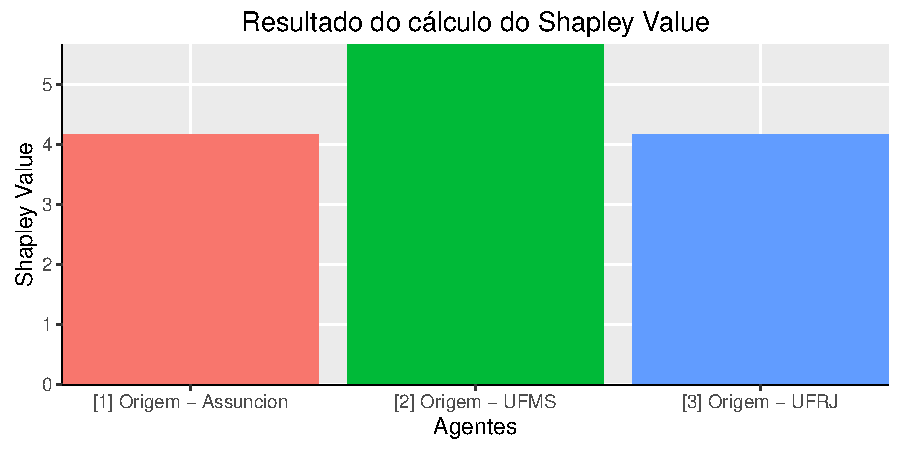
\includegraphics[width=\maxwidth]{figure/unnamed-chunk-4-1} 

}

\caption[Cálculo do Shapley Value]{Cálculo do Shapley Value}\label{fig:unnamed-chunk-4}
\end{figure}


\end{knitrout}


  \texttt{\color{red}...seguem referências para completar seção...}
  \begin{itemize}
    \item Aircraft Landing Fees: A Game Theory Approach \cite{Littlechild.1977}
    \item The Shapley value: essays in honor of Lloyd S. Shapley \cite{Alvin.1988}
    \item Lloyd Shapley's Matching and Game Theory \cite{Serrano.2013}
    \item Cooperative Game Theory and Applications: Cooperative Games Arising from Combinatorial Optimization Problems \cite{Curiel.2013}
    \item On axiomatizations of the Shapley value for assignment games \cite{Brink.2015}
  \end{itemize}

% ----------------------------------------------------------
% Completar artigo
% ----------------------------------------------------------
\section{\texttt{\color{red}...seguem referências para completar artigo...}}

Definição de um jogo cooperativo.

\begin{equation}
  \label{eq:conceitoTJC}
  \left \{ 
    \emph{x} \in \Re^{\emph{n}} \mid f\left ( x,S \right ) \leq c\left ( S \right ), \forall \emph{S} \subseteq \emph{N}
  \right\}
\end{equation}


  \texttt{\color{red}...seguem referências para completar seção...}
  \begin{itemize}
    \item Theory of games and economic behavior \cite{Neumann.1947}
    \item Social choice and individual values \cite{Figueiredo.1994}
    \item Teoria dos Jogos Cooperativos: Conceitos Fundamentais \cite{Moreira.2002}
    \item Teoria Dos Jogos \cite{Fiani.2006}
    \item Bayesian learning in negotiation \cite{Zeng.1998}
    \item Teoria dos Jogos \cite{Tavares.2009}
    \item Teoria dos Jogos \cite{Bierman.2010}
    \item Cooperação e Conflito \cite{Fiani.2011}
    \item Teoria dos Jogos: Crenas, Desejos e Escolhas \cite{Paula.2014}
    \item A Way to Play Claims Problems \cite{Gimenez.2014}
    \item Teoria dos Jogos \cite{Fiani.2015}
    \item Entrevista com Bruce Bueno de Mesquita \cite{Mesquita.2012}
    \item Linearity of unrestrictedly transferable utilities \cite{Aumann.1960}
    \item Introduction to the Theory of Cooperative Games \cite{Peleg.2007}
    \item Game Theory Cooperative Games with Transferable Utility \cite{Peters.2008}
    \item A cooperative game approach to optimal saving theory: Toward a constitution for savings \cite{Forte.1994}
    \item Water Costs Allocation in Complex Systems Using a Cooperative Game Theory Approach \cite{Sechi.2013}
    \item Cooperative Game Theory in Sports \cite{Manuel.2013}
    \item An intersection theorem in TU cooperative game theory \cite{Albeniz.2004}
    \item Axiomatization in cooperative game theory \cite{yakov.2005}
    \item Applying cooperative game theory to power relations \cite{Wiese.2009}
    \item Cooperative game theory and its insurance applications \cite{Lemaire.1993}
    \item A novel cooperative spectrum sensing method based on cooperative game theory \cite{KaitianCao.2010}
    \item A cooperative game theory analysis for transmission loss allocation \cite{Lima.2008}
    \item Social and Economic Networks in Cooperative Game Theory \cite{Ray.2002}
    \item Game theory in cooperative communications \cite{Yang.2012}
    \item Allocation of Unit Start-Up Costs Using Cooperative Game Theory \cite{Hu.2006}
    \item Compromise values in cooperative game theory \cite{Tijs.1993}
    \item Cooperative advertising, game theory and manufacturer--retailer supply chains \cite{Xie.2006}
    \item Estimation of price policies in Senegal An empirical test of cooperative game theory \cite{Beghin.1991}
    \item Information sharing in DEA: A cooperative game theory approach \cite{Lozano.2012}
    \item Quality of service provisioning in worldwide interoperability for microwave access networks based on cooperative game theory \cite{Jiao.2011}
    \item A conceptual application of cooperative game theory to liner shipping strategic alliances \cite{Song.2002}
    \item Using cooperative game theory to optimize the feature selection problem \cite{Sun.2012}
    \item Game Theory as a Theory of a Conflict Resolution - A Shapley Value for Cooperative Games with Quarrelling \cite{Rapoport.1974}
    \item Introduction to Game Theory - N-Person Cooperative Games \cite{Morris.1994}    
    \item Supplier bidding strategy based on non-cooperative game theory concepts in single auction power pools \cite{Kang.2007}
    \item Aplicação de Teoria de Jogos à Alocação de Capacidade Firme em um Sistema Térmico \cite{Ayala.2008}
    \item Value Solutions in Cooperative Games \cite{Mccain.2013} 
    \item Cooperative Games, Solutions and Applications \cite{Driessen.2013}
    \item A Teoria dos Jogos Aplicada ao Processo Penal \cite{Rosa.2014}
    \item Towards a theory of supply chain management: the constructs and measurements \cite{Chen.2004}
    \item Game Theory in Supply Chain Analysis \cite{Cachon.2004}
    \item Supply Chain Games: Operations Management and Risk Valuation \cite{kogan.2007}
    \item Cooperation: Game-Theoretic Approaches \cite{Hart.2012}
    \item Quantitative Methods in Supply Chain Management: Models and Algorithms \cite{Christou.2012}
    \item Cooperation in an HMMS-type supply chain: A management application of cooperative game theory \cite{Dobos.2010b}
  \end{itemize}

\section{Nucleolus}

\subsection{Conceito}

  \texttt{\color{red}...seguem referências para completar seção...}
  \begin{itemize}
    \item The Nucleolus of a Characteristic Function Game \cite{Schmeidler.1969}
    \item Geometric Properties of the Kernel, Nucleolus, and Related Solution Concepts \cite{Maschler.1979}
    \item Game theoretic analysis of a bankruptcy problem from the Talmud \cite{Aumann.1985}
    \item Game Theory (An Introduction) \cite[p.~219--307]{Barron.2007}
    \item Collective Rationality: Equilibrium in Cooperative Games \cite{Weirich.2009}
    \item Prática na Teoria. Aplicações da Teoria dos Jogos e da Evolução aos Negócios \cite{Marinho.2011}
    \item Common mistakes in computing the nucleolus \cite{Guajardo.2015}
    \item O Dilema do Prisioneiro desde Hegel até Lacan: Tomo 1 \cite{Faveret.2015}
  \end{itemize}

\subsection{Aplicação no estudo de caso}

\subsection{Implementac{c}ão computacional para o estudo de caso}


\section{Análise comparativa}

  \texttt{\color{red}...seguem referências para completar seção...}
  \begin{itemize}
    \item Comparative cooperative game theory \cite{Ichiishi.1990}
    \item A cooperative game in search theory \cite{Hohzaki.2009}
  \end{itemize}

% ---
% Finaliza a parte no bookmark do PDF, para que se inicie o bookmark na raiz
% ---
\bookmarksetup{startatroot}% 
% ---

% ---
% Conclusão
% ---
\section{Conclusão}


\begin{citacao}
  Podemos ter uma consciência difusa dos demônios que nos espreitam lá fora. Podemos até estar bastante preocupados com eles. Mas, na realidade, não temos ideia de quantos são e de quando podem atacar \cite{Nate.2012}.
\end{citacao}

\begin{citacao}

[...] toda medição e todo número do mundo real tem um quê de imprecisão, de incerteza. Trata-se de um reflexo imperfeito da realidade. Números são sempre impuros: uma mescla de verdade, erro e incerteza \cite{Seife.2012}.

\end{citacao}


\begin{citacao}
$\left [ ... \right ]$ os objetos primários de nossas percepções morais são as ações de outros homens; além disso, nossos juízos morais sobre nossa própria conduta são apenas aplicações, sobre nós mesmos, de decisões já proferidas a respeito da conduta do nosso próximo \cite{Smith.1999}.
\end{citacao}

\begin{citacao}
  A teoria dos jogos parte do ponto que as pessoas estão buscando o que é bom para elas. O que não parece ser tão chocante embora controverso para muitas pessoas: somos interessados em nós mesmos. E para buscar o que é melhor para si ou o que imaginamos ser melhor, as pessoas têm valores --- elas identificam o que querem e o que não querem \cite[min.~2:17--2:37]{MesquitaTED.2009}. 
\end{citacao}


\begin{citacao}
As paixões podem nos motivar a agir, mas nem sempre são suficientes para prevalecer sobre todas as razões; da mesma forma, as razões, sozinhas, não são tão fortes que garantam que uma ação aconteça. Algumas vezes é preciso um \textbf{acordo} para resolver os nossos dilemas do prisioneiro \emph{internos}, o que envolve a possibilidade de cooperação na escolha que temos de fazer ao longo do tempo entre "prêmios", tais como recompensas, punições e sentimentos de culpa \cite[p.~132]{Pimentel.2007}.
\end{citacao}


  \texttt{\color{red}...seguem referências para completar seção...}
  \begin{itemize}
    \item O andar do bébado \cite{Mlodinow.2009}
    \item Os n\'umeros (não) mentem: Como a matemática pode ser usada para enganar você \cite{Seife.2012}
    \item O sinal e o ruído \cite{Nate.2012}
    \item R{á}pido e devagar: Duas formas de pensar \cite{Kahneman.2012}
    \item Subliminar: Como o inconsciente influencia nossas vidas \cite{Mlodinow.2013}
    \item O poder do h{á}bito: Por que fazemos o que fazemos na vida e nos neg{ó}cios \cite{Duhigg.2012}
    \item O sinal e o ruído \cite{Nate.2012}
  \end{itemize}

\section{*Trabalhos futuros}

  \texttt{\color{red}...seguem referências para completar seção...}
  \begin{itemize}
    \item Games with incomplete information played by ''Bayesian'' players part II. Bayesian equilibrium points \cite{Harsanyi.1968}
    \item Equilibrium points in n-person games \cite{Nash.1950}
    \item Two-person cooperative games \cite{Nash.1953}
    \item Quantum games \cite{JoseFigueiredo.2004}
    \item Quantum games and quantum strategies \cite{Eisert.1999}
    \item Nash equilibria in quantum games with generalized two-parameter strategies \cite{Flitney.2007}
    \item Quantum cooperative games \cite{Iqbal.2002},\cite{Dai.2004}
    \item A probabilistic approach to quantum Bayesian games of incomplete information \cite{Iqbal.2014}
    \item Social optimality in quantum Bayesian games \cite{Azhar.2015}
  \end{itemize}

% ----------------------------------------------------------
% ELEMENTOS PÓS-TEXTUAIS
% ----------------------------------------------------------
\postextual

% ---
% Título e resumo em língua estrangeira
% ---

% \twocolumn[    		% INICIO DE ARTIGO EM DUAS COLUNAS

% ]  				        % FIM DE ARTIGO EM DUAS COLUNAS
% ---

% ----------------------------------------------------------
% Referências bibliográficas
% ----------------------------------------------------------
\bibliography{references}

\end{document}

% ----------------------------------------------------------
% Glossário
% ----------------------------------------------------------
%
% Há diversas soluções prontas para glossário em LaTeX. 
% Consulte o manual do abnTeX2 para obter sugestões.
%
%\glossary

% ----------------------------------------------------------
% Apêndices
% ----------------------------------------------------------

% ---
% Inicia os apêndices
% ---
\begin{apendicesenv}

% ----------------------------------------------------------
\chapter{}
% ----------------------------------------------------------

\end{apendicesenv}
% ---

% ----------------------------------------------------------
% Anexos
% ----------------------------------------------------------
\cftinserthook{toc}{AAA}
% ---
% Inicia os anexos
% ---
%\anexos
\begin{anexosenv}

% ---
\chapter{}
% ---

\end{anexosenv}
